\documentclass[brudnopis]{xmgr}

\setmainfont[Numbers=OldStyle,Mapping=tex-text]{Minion Pro}
\setsansfont[Numbers=OldStyle,Mapping=tex-text]{Myriad Pro}

\usepackage{listings}
\usepackage{xcolor}
\usepackage{fontspec}
\usepackage{minted}

\lstdefinestyle{sharpc}{language=[Sharp]C, frame=lr, rulecolor=\color{blue!80!black}}

\wersja   { }

\author   {Wojciech Denejko}
\nralbumu {214\,300}
\email    {deneyw@gmail.com}

\title    {Rozpoznawanie tekstu w aplikacjach mobilnych}
\date     {2017}
\miejsce  {Gdańsk}

\opiekun  {dr Tomasz Borzyszkowski}

\begin{document}

% streszczenie
\begin{abstract}
  Niniejsza praca ma na celu stworzenie aplikacji rozpoznającej litery oraz cyfry pisane odręcznie, która charakteryzuje się kompatybilnością z systemami \emph{iOS} oraz \emph{Android}. Do wytworzenia aplikacji zostanie użyte narzędzie \emph{Xamarin}, które służy do tworzenia aplikacji wieloplatformowych. Zbadane zostaną różne metody połączenia technologii wieloplatformowej z istniejącymi rozwiązaniami OCR. Przedstawiona konwolucyjna sieć neuronowa zaprezentuje klasyfikacje liter alfabetu oraz cyfr. Zostaną przeprowadzone badania pokazujące przewagę konwolucyjnych sieci neuronowych nad innymi algorytmami uczenia maszynowego.
  
  Integralną częścią pracy jest aplikacja ImageResizer, która pozwala na przygotowanie modelu danych z podzielonego na poszczególne znaki oraz cyfry zbioru danych.
  
\end{abstract}

% słowa kluczowe
\keywords{C\#,
 Xamarin,
 .NET,
 Uczenie maszynowe,
 Sieci neuronowe,
 kNN,
 Random Forest,
 Konwolucyjne sieci neuronowe,
 OpenCV
 }

% tytuł i spis treści
\maketitle

% wstęp
\introduction
	Rozpoznawanie tekstu w aplikacjach mobilnych w dzisiejszych czasach to problem zyskujący na popularności każdego dnia, ponieważ istniejąca technologia pozwala na przedstawianie tego problemu jako łatwy do rozwiązania. Oprogramowania służące do rozpoznawania tekstu posiadają skuteczność (\emph{ang. accuracy}), która w niektórych wypadkach jest nawet równa 100\% prawidłowo rozpoznanego tekstu. Niestety, gotowe rozwiązania są najczęściej płatne lub brak w nich możliwości poszerzania zbioru danych tak, aby zmodyfikować narzędzie pod własne potrzeby.
	
	Najpopularniejsze istniejące biblioteki służące do rozpoznawania tekstu korzystają między innymi z własnych modeli sieci neuronowych oraz ściśle dobranego zbioru danych treningowych. Firmy takie jak \emph{Microsoft}, \emph{Google} oraz \emph{Amazon} rywalizują ze sobą, udostępniając programistom ich własne narzędzia umożliwiające rozpoznawanie tekstu. Działają one na danych, które te firmy utrzymują w swoich bankach danych, a więc daje to wysokie korzyści. Niestety, w przypadku pisma odręcznego. Wyniki pracy z gotowymi rozwiązaniami są co najmniej średnie, a czasami niemożliwe jest przeprowadzenie rozpoznania pojedynczej litery.
	
	Autor w pracy opisał i przedstawił najpopularniejsze metody klasyfikacji znaków pisma odręcznego, czyli algorytmy oraz gotowe rozwiązania firm trzecich, takie jak:
\begin{itemize}
\item
K-najbliższych sąsiadów
\item
Random forest
\item
Sieci neuronowe
\item
TesseractAPI
\item
Microsoft Computer Vision API
\end{itemize}
\newpage

	Xamarin\cite{15} to platforma deweloperska służąca do tworzenia natywnych aplikacji mobilnych dla systemów iOS, Android oraz Windows, za pomocą wspólnej technologii .NET i języka C\#\cite{4} . Dzięki temu możliwe jest uzyskanie do stu procent wspólnego kodu między platformami Android oraz iOS. Aplikacje napisane przy użyciu technologii Xamarin\cite{15} i C\# mają pełny dostęp do interfejsów\cite{20}, API oraz możliwość tworzenia natywnych interfejsów użytkownika. W pracy zostanie udostępniona aplikacja implementująca wszystkie algorytmy oraz gotowe rozwiązania.
  
  Celem pracy jest  zbadanie istniejących rozwiązań służących do rozpoznawania tekstu oraz stworzenie sieci neuronowej pozwalającej na klasyfikację znaków pisanych charakterystycznych dla współczesnego języka polskiego. Dane pozwalające na przeprowadzenie wymaganego treningu sieci neuronowej zostały udostępnione przez portal NIST.GOV\cite{7}. Zbiór Special Database 19 zawiera podzielone na klasy grupy liter od A do Z oraz cyfry od 0 do 9. Następnie zostało swtorzone narzędzie do odczytywania znaków i zapisania ich jako model danych\cite{2}.
  
  W rozdziale pierwszym autor opisze zastosowanie wymienionych algorytmów, a następnie przedstawi implementacje oraz szczegółowy opis działania konwolucyjnej sieci neuronowej. Rozdział drugi szczegółowo obrazuje przekrój istniejących technologii i bibliotek dostępnych w większości na licencji open source. Trzeci rozdział opisuje przeprowadzone badania, które mają na celu udowodnienie, iż implementacja sieci neuronowej autora osiąga lepsze rezultaty, niż opisane narzędzia oraz klasyfikatory zawarte w pracy. Ostatni rozdział zawiera podsumowanie i wnioski.

\chapter{Rozpoznawanie tekstu w aplikacjach wieloplatformowych}

OCR\cite{20} (ang. Optical Character Recognition) jest to technika lub część oprogramowania służąca do rozpoznawania znaków oraz całych tekstów zapisanych w pliku graficznym prezentowanym za pomocą pionowo-poziomej siatki odpowiednio kolorowanych pikseli. Przykładem takiej grafiki jest zdjęcie z aparatu cyfrowego. 

Niegdyś pojęcie rozpoznawania znaków oznaczało samą klasyfikacje ciągów znaków drukowanych, które są łatwiejszym problemem do rozwiązania a dziś również pisma odręczne oraz cechy formatowania, takie jak krój pisma lub układy tabelaryczne (formularze).

Techniki OCR są głównie wykorzystywane do cyfryzacji zasobów bibliotek, a także jako ułatwienie przy odczytywaniu dokumentacji napisanych pismem odręcznym. W aplikacjach mobilnych rozpoznawanie znaków pomaga w takich zadaniach jak tworzenie notatek, a następnie tłumaczenie ich na tekst drukowany. Niestety, w obu przypadkach istniejące rozwiązania OCR nie są tak skuteczne jak człowiek, zatem w przypadkach trudności z klasyfikacją znaku lub fragmentu tekstu niezbędna jest weryfikacja wyniku przez człowieka celem uniknięcia błędu.

Postęp w metodach OCR jest bardzo widoczny, gdyż w obecnych czasach produkty potrafią rozpoznawać mało dokładne zdjęcia tekstu, na przykład wykonane telefonami komórkowymi z szumami na obrazkach, z tekstem napisanym pod nienaturalnymi kątami w wielu językach, pozostaje jednak problem rozpoznawania znaków pisma odręcznego.

Rozpoznawanie pisma jest możliwe dzięki zastosowaniu metod z dziedziny rozpoznawania wzorców, czyli pola badawczego w obrębie uczenia maszynowego. Metoda ta może być definiowana jako działanie polegające na pobieraniu danych i podejmowaniu dalszych czynności zależnych od kategorii, do której należą te dane. By odpowiednio wyodrębnić poszczególne znaki z obrazu używane są biblioteki pozwalające na profesjonalną obróbkę zdjęć pod zastosowania w celach uczenia maszynowego. Przykładem takiej biblioteki jest OpenCV\cite{21}. Po wyodrębnieniu potrzebnych informacji na temat danego znaku obrazy są klasyfikowane jako poszczególne litery. Zwykle w tym procesie używane są sieci neuronowe.

Kompletny system rozpoznawania wzorców składa się z:
\begin{itemize}
\item
Zbioru danych, które oferują możliwość klasyfikacji lub opisu
\item
Mechanizmu wydobywania cech, które najlepiej charakteryzują i separują daną klasę, do której dany element zbioru danych należy
\item
Mechanizmu przekształcenia elementu zbioru w symboliczną informację, łatwiejszą do wykorzystania przez algorytm
\item
Schematu decyzyjnego lub schematu opisu, który realizuje właściwą część procesu klasyfikacji w oparciu o wydobyte i przekształcone cechy obiektu.
\end{itemize}

\section{Przedstawienie problemu}

Wsród istniejących rozwiązań mogących służyć jako narzędzie potrzebne do wytworzenia aplikacji mobilnej, która rozpozna polskie znaki pisma odręcznego nie istnieje łatwy sposób zastosowania rozwiązania pozwalającego na skuteczną klasyfikację polskiego pisma. Brakuje również dostępnych danych wymaganych do skutecznej klasyfikacji w oparciu o przekształcone informacje. Aby rozwiązać ten problem należy stworzyć zbiór treningowy lub rozszerzyć istniejący zbiór o znaki alfabetu charakterystyczne dla danego języka.

Dostępne biblioteki na rynku, takie jak TesseractAPI\cite{10} oraz Microsoft Computer Vision API\cite{9} oferują wysoką skuteczność w rozpoznawaniu polskich oraz angielskich obrazów tekstu drukowanego lecz zarazem brak możliwości rozpoznawania pisma odręcznego. Wymagane jest więc stworzenie systemu rozpoznawania wzorców, który pozwalałby na skuteczną klasyfikacje znaków pisma odręcznego.

Kolejnym problemem są znacząco ograniczone zasoby urządzeń mobilnych. Systemy rozpoznawania wzorców wymagają mocy obliczeniowej potrzebnej do przekształcenia obrazów w postać pozwalającą na wyodrębnianie cech, a następnie przeprowadzenie procesu klasyfikacji. Rozwiązaniem tego problemu jest wykorzystanie systemu rozpoznawania wzorców jako serwisu internetowego działającego w oparciu o architekturę REST\cite{5}.

\section{Sposób wytworzenia zbioru treningowego}

Zbiór treningowy\cite{19} jest kontenerem krotek (przykładów, obserwacji, próbek), będących lista właściwości atrybutów opisowych (tzw. deskryptorów) i wybranego atrybutu decyzyjnego (ang. class label attribute). Głównym jego celem jest zbudowanie formalnego modelu zwanego klasyfikatorem. Wynikiem procesu klasyfikacji jest pewien otrzymany model (klasyfikator), który przydziela każdemu przykładowi wartość atrybutu decyzyjnego w oparciu o właściwości pozostałych atrybutów.

W przypadku systemu rozpoznawania wzorów zbiorem treningowym są zdjęcia obrazów zawierajace odpowiednio wszystkie litery polskiego alfabetu oraz cyfry. Wszystkie zdjęcia liter, które istnieją w zbiorze należy przeformatować do postaci najlepiej rozumiana przez wykorzystywane algorytmy.

Do transformacji zdjęć zastosowano EmguCV\cite{18}. Jest to wieloplatformowa implementacja (ang. wrapper) w technologii .NET biblioteki OpenCV, pozwalająca na wykorzystanie funkcjonalności OpenCV\cite{21} w środowisku .NET we wszystkich jego językach programowania, takich jak C\#, VB, F\#\cite{1}. Można ją zainstalować używając menadżera pakietów Nuget w programie Visual Sutdio, Xamarin Studio lub Unity, a więc jest również kompatybilna z platformami mobilnymi Android oraz iOS.

Transformacja zdjęcia przebiega następująco:
\begin{itemize}
\item
Odczytaj zdjęcie w formacie .png
\item
Przeprowadź konwersje kolorów RGB na odcienie szarości
\item
Przetwórz obraz do formatu 28 x 28 piksele
\item
Odczytaj stopień jasności każdego piksela w skali od 0 do 255 i zapisz je w tablicy
\end{itemize}

\begin{figure}[!tbh]
\centering
\includegraphics[width=.6\hsize]{fig/ą}
\caption{Przykład zdjęcia znaku, \emph{Źródło: Opracowanie własne}}
\end{figure}
Rezultatem działania programu do konwersji zdjęć jest plik train.csv. Zawiera on 785 kolumn. Pierwsza kolumna, nazwana "label", określa znak, który jest narysowany. Reszta kolumn zawiera informacje na temat jasności każdego piksela.

Każda kolumna w zbiorze treningowym ma ustawioną nazwę pixelx, gdzie x jest liczbą między 0 a 783. By znaleźć dany piksel na obrazie, należy rozłożyć x jako x = a * 28 + b, gdzie a i b to liczby między 0 a 27. Wtedy pixelx jest umieszczony w a-tym rzędzie b-tej kolumnie w macierzy 28 x 28, indeksowanej od zera. Na przykład, pixel31 wskazuje na piksel w czwartej kolumnie od lewej i drugim wierszu od góry. Tak, jak pokazane na diagramie poniżej:

\begin{lstlisting}
000 001 002 003 ... 026  027
028 029 030 031 ... 054  055
 |   |   |   |  ...  |    |
728 729 730 731 ... 754  755
768 769 770 771 ... 782 783 
\end{lstlisting} 
\newpage

Fragment aplikacji pozwalającej na stworzenie modelu danych załączony poniżej:

\begin{minted}{csharp}
var csv = new StringBuilder();
var csv2 = new StringBuilder();
var fileName = files[i].DirectoryName
               .Replace(imagesPath + @"\", string.Empty);
csv.Append(fileName);
csv.Append(',');
var originalImage = new Image<Gray, byte>(files[i].FullName)
                    .Not();
var img = originalImage.Resize(28, 28, Inter.Linear);
for (var k = 0; k < img.Height; k++)
{
    for (var j = 0; j < img.Width; j++)
    {
       csv.Append(img[k, j].Intensity);
       csv.Append(',');
    }
}
csv2.AppendLine(csv.ToString());
File.AppendAllText(csvFilePath, csv2.ToString());
\end{minted}

Pełna wersja programu znajduje się w dołączonej dokumentacji na płycie CD w folderze pod nazwą ImageResizer

\section{Algorytm k-NN}

Algorytm k-najbliższych sąsiadów (ang. k nearest neighbours)\cite{2}\cite{11} - algorytm regresji nieparametrycznej najczęściej używany w statystyce do prognozowania pewnej wartości zmiennej losowej.
\newpage

Założenia:
\begin{itemize}
\item
Dany jest zbiór teningowy, który stworzony został w oparciu o narzędzie TraningSetGenerator.
\item
Dana jest obserwacja C, zawierająca wektor zmiennych $pixel_{0}$ ... $pixel_{1024}$, dla której chcemy prognozować wartość zmiennej objaśnianej label.
\end{itemize}	

Algorytm działa następująco:
\begin{itemize}
\item
Porównaj wartości zmiennych objaśniających dla obserwacji C, z każdym wektorem w zbiorze treningowym.
\item
Wybierz k (ustalonej z góry liczby) najbliższych do C obserwacji ze zbioru treningowego.
\item
Uśrednienij wartości zmiennej objaśnianej dla wybranych obserwacji, w wyniku czego uzyskujemy prognozę.	
\end{itemize}	
     
Poniższy przykład demonstruje problem klasyfikacji przy użyciu algorytmu kNN,.Obiekt zaznaczony kołem dla k najbliższych sąsiadów równe 2, zostanie sklasyfikowany jako trójkąt. Natomiast jeżeli do klasyfikacji zostanie użytych 3 najbliższych sąsiadów obiekt zostanie sklasyfikowany jako kwadrat.

\begin{figure}[!tbh]
\centering
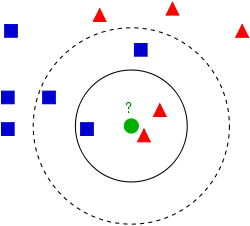
\includegraphics[width=.4\hsize]{fig/knn}
\caption{Przykład problemu k-NN, \emph{Źródło: http://shyamalapriya.github.io/digit-recognition-using-k-nearest-neighbors/}}
\end{figure}
\newpage

Dla k = 3, niewiadoma oznaczona zielonym punktem będzie sklasyfikowana jako czerwony trójkąt w oparciu o trzech najbliższych sąsiadów, jednak jeśli k = 5, zostałaby sklasyfikowana jako niebieski kwadrat ponieważ algorytm działałby w oparciu o pięciu sąsiadów. Najbliżsi sąsiedzi są określani przy pomocy metryki euklidesowej określonej wzorem:

\begin{figure}[!tbh]
\centering
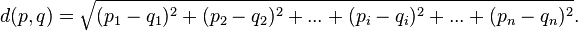
\includegraphics[width=1\hsize]{fig/knn-wzor}
\end{figure}

Fragment przykładowej implementacji powyższego algorytmu, który klasyfikuje przykładowy znak alfabetu dla k = 3 znajduje się poniżej:

\begin{minted}{python}
labeled_images = pd.read_csv('output.csv')
images = labeled_images.iloc[0:5000,1:]
labels = labeled_images.iloc[0:5000,:1]
train_images, test_images, train_labels, test_labels 
= train_test_split(images, labels, train_size=0.8, random_state=0)
knn = KNeighborsClassifier(n_neighbors=3, algorithm="kd_tree")
knn.fit(train_images, train_labels.values.ravel())
print knn.score(test_images,test_labels)
\end{minted}

Pełna implementacja algorytmu k najbliższych sąsiadów jest dołączona w dokumentacji pracy na płycie CD.

\section{Random Forest}
Drzewa decyzyjne to graficzna metoda wspomagania procesu decyzyjnego. Algorytm drzew decyzyjnych jest również stosowany w uczeniu maszynowym do pozyskiwania wiedzy na podstawie przykładów.
\newpage

Koncepcja Bugging polega na budowie ekspertów dla podzbioru zadań. W tym przypadku, ze wszystkich problemów do rozwiązania losowany jest jeden z nich ze zwracaniem podzbioru problemów, a następnie dla tego podzbioru szukany jest ekspert. W algorytmie tym z całego zbioru danych uczących losowany jest podzbiór - przez losowanie ze zwracaniem - i dla tego podzbioru budowany jest model predykcyjny. Następnie po raz kolejny ze zwracaniem losowany jest inny podzbiór wektorów i dla niego budowany jest kolejny model. Całość powtarzana jest k krotnie a na koniec wszystkie zbudowane modele użyte są do głosowania.

Algorytm Random Forest\cite{3}\cite{13} to metoda klasyfikacji polegająca na połączeniu drzew decyzyjnych oraz koncepcji bugging. Tworzy ona wiele drzew decyzyjnych na podstawie losowego zestawu danych. Idaą tego algorytmu polega na zbudowaniu rady ekspertów z losowych drzew decyzyjnych, gdzie w odróżnieniu od klasycznych drzew decyzji, losowe drzewa budowane są ze zbiorów analizowanych cech. Ponadto, poszczególne drzewa z losowych lasów budowane są zgodnie z koncepcją Bugging.

Cechy algorytmu Random Forest:
\begin{itemize}
\item
Działa skutecznie na dużych zbiorach treningowych
\item
Utrzymuje dokładność w przypadku braku danych
\item
Daje oszacowanie, które zmienne są istotne w klasyfikacji
\item
Lasy drzew mogą być zapisane i wykorzystane w przyszłości dla innego zbioru danych
\item
Nie wymaga wiedzy eksperckiej
\end{itemize}

Algorytm działa następująco:
\begin{itemize}
\item
Losujemy ze zwracaniem z n-elementowego zbioru treningowego n wektorów. Na podstawie takiej próby zostanie stworzone drzewo.
\item
W każdym węźle podział odbywa się poprzez wylosowanie bez zwracania m spośród p atrybutów, następnie w kolejnym węźle k spośród m atrybutów
\item
Proces budowania drzewa bez przycinania trwa, jeśli to możliwe do momentu uzyskania w liściach elementów z tylko jednej klasy.
\end{itemize}
\newpage

Proces klasyfikacji:
\begin{itemize}
\item
Dany wektor obserwacji jest klasyfikowany przez wszystkie drzewa i ostatecznie zaklasyfikowany do klasy, w której wystąpił najczęściej.
\item
W przypadku elementów niewylosowanych z oryginalnej podpróby, każdy taki i-ty element zostaje poddany klasyfikacji przez drzewa, w których budowie nie brał udziału. Taki element zostaje następnie przyporządkowany klasie, która osiągana była najczęściej.
\end{itemize}

\begin{figure}[!tbh]
\centering
\includegraphics[width=.6\hsize]{fig/randomforest}
\caption{Diagram przepływu algorytmu Random Forest \emph{Źródło: Opracowanie własne}}
\end{figure}
\newpage

Fragment przykładowej implementacji powyższego algorytmu, klasyfikującego przykładowy znak alfabetu znajduje się poniżej:

\begin{minted}{python}
images = labeled_images.iloc[0:5000,1:]
labels = labeled_images.iloc[0:5000,:1]
train_images, test_images, train_labels, test_labels 
= train_test_split(images, labels, train_size=0.8, random_state=0)
clf = RandomForestClassifier(n_jobs=2).fit(train_images, train_labels.values)
print clf.score(test_images,test_labels)
\end{minted}

Pełna implementacja algorytmu Random Forest jest dołączona w dokumentacji pracy na płycie CD. 

\section{Wielowarstwowe sieci neuronowe}

Siecią neuronową\cite{1}\cite{12} nazywa się programową lub sprzętową strukturę modeli, realizującą obliczenia lub przetwarzającą sygnały poprzez rzędy elementów, zwanych sztucznymi neuronami. Emulują one niektóre spośród zaobserwowanych właściwości biologicznych układów nerwowych. Sztuczne sieci neuronowe są swoistymi systemami inspirowanymi tym, w jaki sposób gęsto połączone między sobą struktury mózgu, odbierają i przetwarzają dane które docierają w różny sposób z otoczenia. Kluczowym elementem jest zatem struktura systemu przetwarzania informacji. Sieć taka składa się z dużej liczby rozlegle połączonych ze sobą elementów przetwarzających, które są powiązane ze sobą ważonymi połączeniami.

Cechą odróżniającą sieci neuronowe od klasyfikatorów realizujących przetwarzanie informacji przy użyciu algorytmów jest umiejetność generalizacji, czyli zdolność uogólniania wiedzy dla nieznanych wcześniej wzorców. Innym atutem jest także zdolność do aproksymacji wartości funkcji wielu zmiennych w przeciwieństwie do interpolacji, która jest możliwa do uzyskania używając przetwarzania algorytmicznego.

Uczenie sieci neuronowych zmienia liczbowe wartości wag znajdujących się pomiędzy neuronami. Następuje to poprzez bezpośrednią ekspozycje rzeczywistego zestawu danych, gdzie algorytm uczący modeluje wagi połączeń. W dziedzinie nauk technicznych sieci neuronowe wykorzystuje się do rozwiązywania między innymi problemów:

\begin{itemize}
\item
Aproksymacji i prognozowania
\item
Klasyfikacji i rozpoznawania
\item
Kojarzenia danych - sieci neuronowe pozwalają zautomatyzować procesy wnioskowania i pomagają wykrywać istotne powiązania między danymi
\item
Analizy danych, czyli poszukiwania związków między danymi
\end{itemize}

Podstawowym elementem sieci neuronowej jest neuron. Jego schemat został opracowany przez McCullocha i Pittsa w roku 1943, został on oparty na schemacie budowy biologicznej komórki nerwowej.

\begin{figure}[!tbh]
\centering
\includegraphics[width=.8\hsize]{fig/budowaneurona}
\caption{Schemat sztucznego neuronu, \emph{Źródło: http://www.cs.put.poznan.pl/rklaus/assn/images/modeln.gif}}
\end{figure}

Do wejść doprowadzane są sygnały z wejść sieci lub neuronów warstwy poprzedniej. Każdy sygnał mnożony jest przez odpowiadającą mu wartość liczbowa zwaną wagą. Wpływa ona na percepcje danego sygnału wejściowego i jego udział w sygnale wyjściowym przez neuron. Waga może być dodatnia lub ujemna a jeżeli nie ma połączenia miedzy neuronami to waga jest równa zero. Zsumowane iloczyny wag i sygnałów są argumentem funkcji zwanej funkcją aktywacji neuronu.
\newpage

Wartość funkcji aktywacji jest wyjściem neuronu i propagowana jest do neuronów warstwy następnej. Może ona przybierać jedną z trzech postaci:
\begin{itemize}
\item
Nieliniową
\item
Liniową
\item
Skoku jednostkowego.
\end{itemize}

Należy zauważyć, iż jest to podział bardziej formalny niż merytoryczny. Różnice funkcjonalne między tymi typami raczej nie występują, natomiast można stosować je naprzemiennie w różnych warstwach sieci.

Najbardziej popularnym typem sieci neuronowej jest sieć wielowarstwowa (ang. Multi-Layer Neural Network). Jej cechą charakterystyczną jest występowanie co najmniej jednej warstwy ukrytej neuronów, pośredniczącej w przekazywaniu sygnałów pomiędzy wejściami a wyjściami sieci.

\begin{figure}[!tbh]
\centering
\includegraphics[width=.8\hsize]{fig/budowasieci}
\caption{Schemat budowy sieci wielowarstwowej, \emph{Źródło: http://galaxy.agh.edu.pl/~vlsi/AI/ex02/pogoda\_files/schemat1\_gif\_1.gif}}
\end{figure}
\newpage

Do rozpoznania polskich znaków pisma odręcznego użyta została sieć posiadająca trzy warstwy:

\begin{itemize}
\item
Warstwa wejściowa sieci składa się z neuronów zawierających informacje na temat każdego piksela. Zbiór treningowy składa się z obrazów 28 x 28 pikseli. Zgodnie z tym założeniem pierwsza warstwa sieci składa się z 784 neuronów. Każdy z nich przechowuje wartość skali szarości piksela, gdzie 0.0 oznacza kolor biały, a 1.0 czarny.
\item
Druga warstwa zawiera n neuronów, liczba n jest używana w kontekscie eksperymentalnym.
\item
Ostatnia warstwa zawiera 36 neurony, ponieważ alfabet składa się z 26 liter, rozpatrywane są zarówno litery oraz cyfry.
\end{itemize}

Poniżej przedstawiony jest fragment implementacji sieci neuronowej z użyciem pakietu scikit-learn\cite{17}. Pełny kod programu znajduje się na dołączonej płycie CD.

\begin{minted}{python}
x0 = x[:split]; x1 = x[split:]
y0 = y[:split]; y1 = y[split:]
mlp = MLPClassifier(solver='sgd', activation='relu',
                    hidden_layer_sizes=(100,30),
                    learning_rate_init=0.3, learning_rate='adaptive', 
                    alpha=0.1, momentum=0.9, 
                    nesterovs_momentum=True,
                    tol=1e-4, max_iter=200,
                    shuffle=True, batch_size=300,
                    early_stopping = False, validation_fraction = 0.15,
                    verbose=True)
mlp.fit(x0,y0)
\end{minted}

\newpage

\section{Konwolucyjne sieci neuronowe - CNN}

Konwolucyjne sieci neuronowe (ang. Convolutional Neural Networks)\cite{14} są podobne do klasycznych sieci neuronowych. Aby dokładnie przeanalizować budowę oraz działanie CNN przedstawiony zostanie problem klasyfikacji dwóch liter X i O. Ten przykład demonstruje charakterystyczne reguły konwolucji.

\begin{figure}[!tbh]
\centering
\includegraphics[width=0.7\hsize]{fig/cnn1}
\caption{Problem klasyfikacji, \emph{Źródło: Opracowanie własne}}
\end{figure}

CNN porównuje obrazy w kawałkach. Każda część nazywana jest cechą (ang. feature). Następnie zdjęcia przeszukiwane są na podobnych pozycjach, aby uzyskać maksymalną liczbę cech wspólnych. Sieci konwolucyjne wykorzystują podobieństwa na obrazach.

\begin{figure}[!tbh]
\centering
\includegraphics[width=0.7\hsize]{fig/cnn2}
\caption{Wybrane cechy i ich odpowiedniki w zdjęciu do klasyfikacji, \emph{Źródło: Opracowanie własne}}
\end{figure}
\newpage

Każdą cechę można scharakteryzować jako mniejsze zdjęcie lub dwuwymiarową tablice wartości. W przypadku litery X, cechami będą ukośne linie i znak krzyża.

\begin{figure}[!tbh]
\centering
\includegraphics[width=.7\hsize]{fig/cnn3}
\caption{Wartości liczbowe pikseli różnych cech, \emph{Źródło: Opracowanie własne}}
\end{figure}

Kiedy rozpatrywany jest nowy obraz, sieć poszukuje cech zdjęcia w każdej możliwej pozycji. Obliczając wartości pasujące do cech tworzymy filtr. Działania matematyczne kryjące się za tym działaniem nazywane są splotem całkowitym. Aby obliczyć parę cech obrazu, należy pomnożyć każdą wartość piksela cechy przez odpowiadający mu piksel danego zdjęcia. Następnie należy dodać wszystkie wyniki z poprzednich operacji i podzielić przez łączną liczbę pikseli cechy. Jeśli oba piksele były białe a ich wartość była reprezentowana przez 1, wynik wynosi 1 - piksel jest biały, w przeciwnym wypadku piksel jest czarny a jego wartość jest równa -1. Jeżeli wszystkie wartości cechy są takie same, wynikiem dodawania i podzielenia przez liczbę pikseli będzie 1.
\newpage

\begin{figure}[!tbh]
\centering
\includegraphics[width=.5\hsize]{fig/cnn4}
\caption{Wynik przykładowej operacji splotu, \emph{Źródło: Opracowanie własne}}
\end{figure}

Następnym krokiem jest powtórzenie operacji splotu na kompletnym obrazie, używając wszystkich dostępnych cech. Wynikiem jest szereg obrazów z filtrami. Na każdym z dostępnych wyników nałożony jest jeden filtr. W konwolucyjnych sieciach neuronowych warstwa ta nazywana jest warstwą konwolucyjną, bądź splotową (ang. convolution layer).

\begin{figure}[!tbh]
\centering
\includegraphics[width=.8\hsize]{fig/cnn5}
\caption{Wynik operacji splotu danej cechy, \emph{Źródło: Opracowanie własne}}
\end{figure}
\newpage


\begin{figure}[!tbh]
\centering
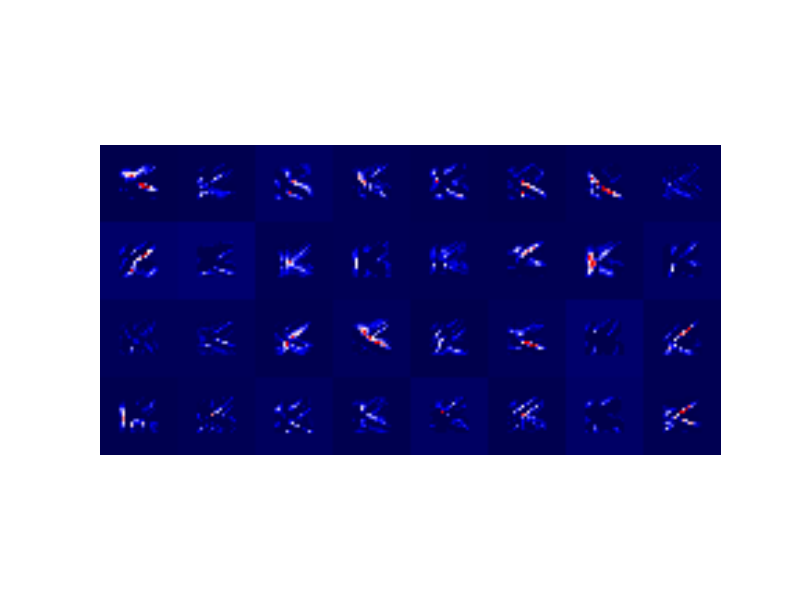
\includegraphics[width=.7\hsize]{fig/figure_1}
\caption{Przykład warstwy konwolucyjnej dla litery k, \emph{Źródło: Opracowanie własne}}
\end{figure}

Kolejnym narzędziem oferowanym przez CNN jest warstwa sumowania (ang. pooling layer). Pooling daje możliwość zmniejszenia dużych obrazów bez utraty ważnych informacji na ich temat. Operacje wykonywane w tej warstwie to podział zdjęcia z poprzedniej warstwy na mniejsze, a następnie pobranie maksimum z danej części. Operacje te należy powtórzyć na całym zdjęciu.

\begin{figure}[!tbh]
\centering
\includegraphics[width=.7\hsize]{fig/cnn6}
\caption{Przykład sumowania, \emph{Źródło: Opracowanie własne}}
\end{figure}
\newpage

Po sumowaniu, wielkość danego zdjęcia jest cztery razy mniejsza. Ponieważ przetrzymywane są wartości maksymalne z każdego okna, przechowywane zostają najlepsze pasujące wartości danej cechy w oknie. To oznacza, że nie ważne jest gdzie pasuje dana cecha do momentu, aż znajdziemy pasującą odpowiedź w oknie.

Dodatkowym narzędziem jest warstwa normalizacyjna (ang. Rectified Linear Units Layer, ReLU). Użycie tej funkcji pozwala ustawić wszystkie ujemne wartości liczbowe na zero. Jeśli wartość jest większa od zero, funkcja ReLU zwróci jeden. To ważny proces w którym wszystkie ujemne wartości zostają zastąpione zerami. Wspomaga to funkcjonowanie sieci, sprawiając, że wszystkie wartości na których wykonywane są operacje są równe 0 lub dodatnie.

\begin{figure}[!tbh]
\centering
\includegraphics[width=.8\hsize]{fig/cnn7}
\caption{Przykład normalizacji danych, \emph{Źródło: Opracowanie własne}}
\end{figure}

Ostatnią możliwą do wykorzystania warstwą sieci jest warstwa FCL (ang. Fully Connected Layer). Jak sama nazwa wskazuje, zadaniem tego poziomu sieci jest połączenie otrzymanych wyników w poprzednich fazach, czyli fazie Splotu, Pooling oraz ReLU. Wynikiem połączenia jest tablica wartości z przedziału od 0 do 1. 
\newpage

W zaprezentowanym przykładzie problem brzmi: Do jakiej kategorii należy znak A przedstawiony na obrazku, X czy O?

Warstwa FCL zbudowana jest z wielu tradycyjnych sieci neuronowych. Zamiast traktować wejście sieci jako dwuwymiarowe tablice, wykorzystywane są tablice jednowymiarowe. Każda wartość otrzymuje końcowy wynik określający, czy na zdjęciu przedstawione jest X - w takim wypadku wynik byłby równy 1 lub kiedy końcowy wynik jest równy 0 odpowiedzią zwróconą przez model jest litera O.

\begin{figure}[!tbh]
\centering
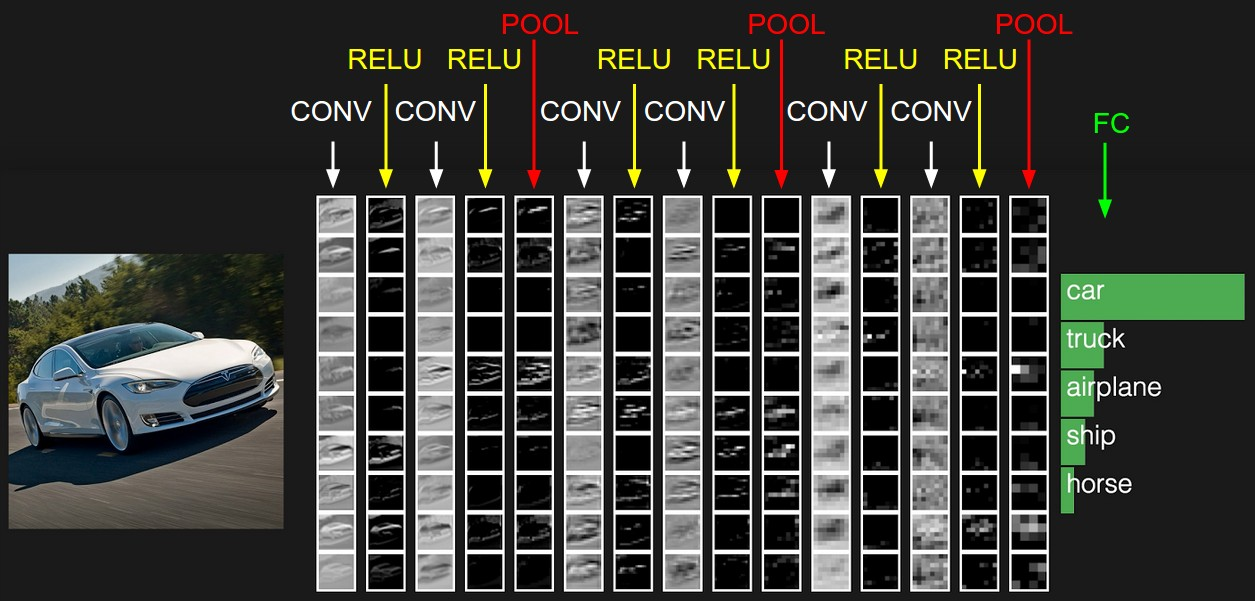
\includegraphics[width=.8\hsize]{fig/convnet}
\caption{Klasyfikacja przykładowego obrazu, \emph{Źródło: http://cs231n.github.io/convolutional-networks/}}
\end{figure}

Podsumowując klasyfikacja przebiega następująco:
\begin{itemize}
\item
Stwórz pierwszą warstwę splotu sieci i wyznacz 10 cech \emph{(ang. feature)} przykładowego zdjęcia,
\item
Wykonaj ReLU, znormalizuj dane,
\item
Następnie ponownie wykonaj krok 1 i 2,
\item
Przeprowadź sumowanie. Zmniejsz wielkość cech,
\item
Kolejnym etapem jest wykonanie kroków od 1 do 4 dwukrotnie,
\item
Po trzykrotnym wykonaniu operacji Pooling, stwórz warstwę FCL i podaj zaproponowane rozpoznania.
\end{itemize}

\chapter{Przegląd bibliotek uczenia maszynowego}
Aby dobrze zobrazować problem rozpoznawania pisma odręcznego w aplikacjach mobilnych, wykorzystanych zostało kilka technologii oraz bibliotek dostępnych w językach programowania Python oraz C\#. Jednocześnie wybrane przykłady demonstrują gotowe implementacje algorytmów, które pozwalają wykorzystywać uczenie maszynowe do własnych potrzeb bez koniecznej wiedzy z zakresu uczenia maszynowego. Takimi technologiami są Microsoft Computer Vision\cite{9} oraz TesseractAPI\cite{10}. Drugim przykładem są biblioteki dostępne do użycia dla programistów uczenia maszynowego, pozwalające na precyzyjne skonfigurowanie dostępnych algorytmów do własnych potrzeb. Są to biblioteki Scikit-learn oraz Tensorflow. Dodatkowo, wykorzystana została biblioteka EmguCV pozwalająca na wykrywanie znaków na zdjęciach oraz odpowiednie formatowanie go na potrzeby stworzenia modelu danych do treningu.

\section{Microsoft Computer Vision API}

Usługi Microsoft Cognitive Services\cite{9} umożliwiają kompilowanie aplikacji z zaawansowanymi algorytmami przy użyciu zaledwie kilku wierszy kodu. Działają one na różnych urządzeniach i platformach, takich jak systemy iOS, Android i Windows. Wciąż są ulepszane i łatwo je skonfigurować. Usług uruchomionych w ramach wyżej wymienionego API jest dokładnie 22. Począwszy od lokalizowania twarzy na zdjęciach, rozpoznawania emocji, wykrywania tekstu na fotografiach, konwertowania mowy na tekst a skończywszy na autosugestii wprowadzanego tekstu prosto z wyszukiwarki Bing.

\begin{figure}[!tbh]
\centering
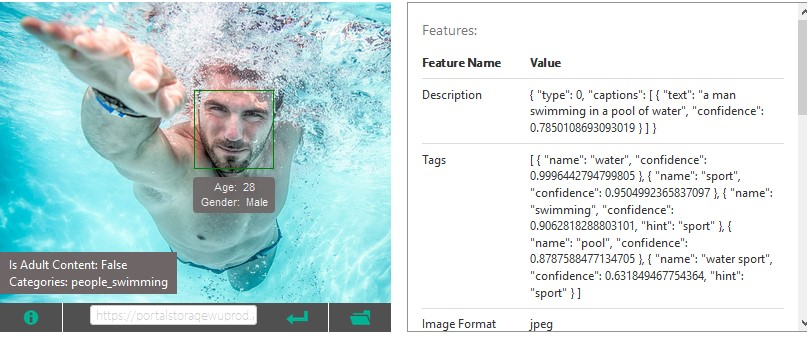
\includegraphics[width=.8\hsize]{fig/mscvapi}
\caption{Przykładowa aplikacja implementująca Computer Vision API, \emph{Źródło: https://www.programmableweb.com/sites/default/files/microsoft\%20computer\%20vision\%20API.jpg}}
\end{figure}
\newpage

Computer Vision API jest system opartym na rozwiązaniach chmurowych firmy Microsoft - Azure. Dostarcza deweloperom dostęp do algorytmów pozwalających na przetwarzanie obrazów i zwracanie informacji na ich temat. Poprzez wysłanie obrazu do serwera algorytmy umieszczone w chmurze firmy Microsoft są w stanie zanalizować kontekst wizualny na wiele różnych sposobów na podstawie wyboru użytkownika.

Ta technologia zawiera między innymi narzędzia do rozpoznawania znaków oraz całych tekstów. Działa ona w 21 językach, dostępny jest również język polski. Usługa posiada możliwość dostosowania kątu nachylenia tekstu, horyzontalnego obrotu osią by rozpoznania dawały lepszy efekt. 

Skuteczność rozpoznanego tekstu zależy od jakości zdjęcia. Nie dokładne rozpoznania mogą być spowodowane dostarczeniem zdjęcia które:

\begin{itemize}
\item
Zawiera odręczne pismo
\item
Jest rozmazane lub czcionka tekstu jest rzadko spotykana
\item
Posiada złożone tła, cienie, odbicia na tekscie
\end{itemize}

Od marca 2017 roku technologia ta pozwala na rozpoznawanie ręcznie pisanego tekstu w języku angielskim. Dostępna jest ona w wersji demonstracyjnej i rozpoznaje jedynie zdjęcia w języku angielskim.

\section{TesseractAPI}

Tesseractjest silnikiem służącym do rozpoznawania znaków. Dostępny jest on na oficjalnej stronie\cite{10}, na zasadzie wolnych źródeł. Może być on używany bezpośrednio lub używając API by wyodrębnić napisane odręcznie bądź też drukowane znaki ze zdjęć. Obsługuje on ponad 20 języków ,w tym też język polski.

Zaletą dostępnego API jest prosta obsługa, brak konieczności posiadania wiedzy z zakresu modelowania algorytmów do uczenia maszynowego oraz gotowe modele języka, które dostępne są do pobrania na stronie projektu.

Wadami tego systemu jest brak możliwości ingerencji w model danych, którymi dysponuje API. Nie ma także możliwości modyfikacji algorytmów, które wykorzystywane są do rozpoznawania znaków. Skutkuje to niską skutecznością rozpoznania znaków pisma odręcznego.

\section{TensorFlow}

Najważniejsze zastosowania TensorFlow\cite{16}, stworzonej przez Google biblioteki sztucznej inteligencji, rozpoznawanie obrazów i mowy, maszynowe tłumaczenia oraz dostarczanie lepszych wyników wyszukiwania w danych. Biblioteka jest otwarta i udostępniona na wolnej licencji Apache 2.0.

Działanie TensorFlow przypomina sposób wykonywania obliczeń za pomocą grafu skierowanego, w którym wierzchołki to matematyczne operacje lub punkty, w których dochodzi do wymiany danych, zaś krawędzie opisują relacje wejścia i wyjścia pomiędzy węzłami, przedstawione w formie dynamicznych macierzy danych, czyli tensorów.

\begin{figure}[!tbh]
\centering
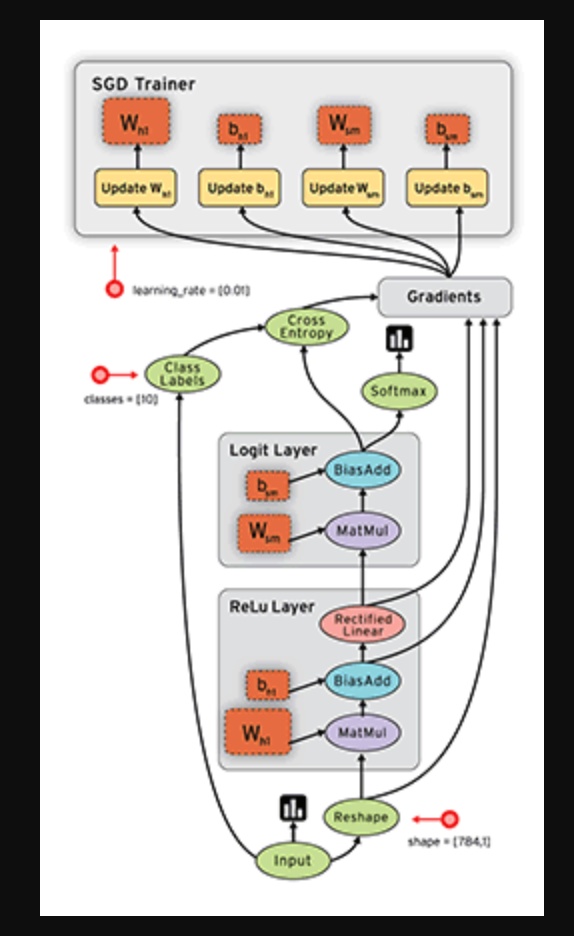
\includegraphics[width=.8\hsize]{fig/tf}
\caption{Graf przedstawiający działanie TensorFlow, \emph{Źródło: https://kimschmidtsbrain.files.wordpress.com/2015/10/tensorflow-flow.jpg}}
\end{figure}
\newpage

Biblioteka oferowana przez firmę Google pozwala na obliczenia numeryczne z wykorzystywaniem takich grafów. Można tu korzystać z ogromnych klastrów superkomputerowych, stacji roboczych z wieloma procesorami graficznymi, a nawet wielordzeniowych mobilnych procesorów w smartfonach.

W badaniach nad problemem rozpoznawania znaków, biblioteka TensorFlow została użyta by stworzyć Splotową  Sieć Neuronową.  Sposób wykonywania operacji na macierzach, elastyczność oraz bogata dokumentacja pozwalają na proste zamodelowanie sieci, która  potrafi rozpoznać litery i cyfry pisane odręcznie z wysoką skutecznością.

\section{Scikit-learn}

Scikit-learn\cite{17} is biblioteką dostępną w języku Python. Służy ona do uczenia maszynowego, oferuje ona szereg algorytmów. Biblioteka zbudowana jest na podstawie SciPy, który jest wymaganym elementem do instalacji i używania scikit-learn. W stos SciPy wchodzą biblioteki:

\begin{itemize}
\item
NumPy - dostarcza on n-wymiarowe tablice
\item
SciPy - służy do wykonywania obliczeń naukowych
\item
Matplotlib - narzędzie do rysowania grafów 2D/3D
\item
Pandas - struktury oraz analiza danych
\end{itemize}

Celem autorów biblioteki było dostarczenie solidnego i dobrze wspomaganego przez społeczność zestawu narzędzi, które działałyby na systemach produkcyjnych. To oznacza,  prostotę, wysoką jakość kodu, dokumentację oraz wysoką wydajność biblioteki.

Scikit-learn oferuje dużą liczbe klasyfikatorów takich jak:
\begin{itemize}
\item
Algorytm k-najbliższych sąsiadów
\item
Drzewa decyzyjne
\item
Random forest
\item
Regresja liniowa
\item
Sieci neuronowe
\end{itemize}

Na ten moment. Biblioteka nie oferuje wsparcia dla własnych modeli sieci neuronowych oraz wykorzystywania klastrów procesorów graficznych.

\section{EmguCV}

EmguCV\cite{18} jest wieloplatformową implementacją biblioteki OpenCV służącą do przetwarzania zdjęć. Pozwala ona na wywoływanie funkcji OpenCV z poziomu .NET oraz języki programowania, które są wspierane takie jak C\#, VC++, IronPython czy F\#. Implementacja ta może być skompilowana z poziomu Visual Studio, Xamarin Studio oraz Unity. Działa na platformach Windows, Linux, Mac OS X, iOS, Android oraz Windows Phone.

Zaletami użycia EmguCV jest przede wszystkim możliwość implementacji na wielu platformach używając jednej technologi, gdyż EmguCV jest napisna w języku C\#. To oznacza że może być kompilowana za pomocą Mono, czyli kompilatora C\# dostępnego pod platformami Linux oraz Mac OS X. Dzięki temu przy użyciu platformy Xamarin oraz EmguCV wszystkie operacje związane z obróbką zdjęcia i przygotowaniem go do klasyfikacji mogą zostać wykonane z poziomu aplikacji. Jest to ważny aspekt, gdyż w przypadku ograniczonych zasobów koszt przygotowania zdjęcia do klasyfikacji jest wysoki.

\chapter{Przeprowadzone badania}

Aby przeprowadzić badania wskazujące czy przedstawiona propozycja konwolucyjnej sieci neuronowej autora osiąga lepsze wyniki rozpoznania od innych, opisanych w pracy rozwiązań, stworzona została wieloplatformowa aplikacja mobilna, która po narysowaniu dowolnego znaku lub cyfry podejmuje próbę rozpoznania.
Porównane zostaną implementacje Microsoft Computer Vision API\cite{9}, TesseractAPI\cite{10} oraz Webservice'u\cite{5} stworzonego przez autora, który rozpoznanie określa na podstawie modelu sieci CNN\cite{14}.

Podjęta zostanie również próba porównania treningu modeli o różnym rozmiarze jednego znaku. Punktem wejściowym do pomiaru będzie pełny model danych około 1mln zdjęć cyfr i liter. Przedstawione zostaną warianty tego modelu posiadające inną liczbę elementów, bądź inny rozmiar zdjęć.

\section{Xamarin}

Xamarin\cite{15} pozwala na tworzenie natywnych aplikacji Android/iOS z wykorzystaniem języka C\# i platformy .NET. Same aplikacje tworzymy w Visual Studio lub Xamarin Studio, a możemy do tego podejść na dwa sposoby: Xamarin.Native lub Xamarin.Forms. Xamarin od zeszłego roku jest dostępny dla wszystkich zainteresowanych, dzięki jego przejęciu przez Microsoft. Natomiast sam kod źródłowy Xamarina został udostępniony na GitHub.

Kompilator Xamarin.iOS kompiluje aplikacje AOT(ang. Ahead-of-time)  do natywnego kodu dla ARM, który jest uruchamiany bezpośrednio na iPhone’ach. Natomiast kompilator Xamarin.Android kompiluje do języka IL (Intermediate Language). Następnie by uruchomić aplikację, korzysta z JIT (ang. Just-in-time). Dzięki tym zabiegom, Xamarin jest transparentny dla docelowych systemów mobilnych, tworząc natywne, w pełni funkcjonalne aplikacje.

W Xamarin.Forms\cite{6} można pisać kod na dwa sposoby, w tzw. code behind w C\# lub za pomocą XAML. Drugi sposób dla osób z doświadczeniem w WPF jest bardzo wygodnym rozwiązaniem. Xamarin.Forms tzw. warpery na natywne kontrolki. Oznacza to, że np. odwołując się do kontrolki Label w Formsa-ch odwołujemy się do ich natywnych odpowiedników w poszczególnych platformach pisząc tylko jeden kod. Ponadto kontrolki Xamarin.Forms są w pełni edytowalne i konfigurowalne tzn. w przypadku gdy czegoś brakuje, można poszukać gotowego rozwiązania lub stworzyć własne.

\begin{figure}[!tbh]
\centering
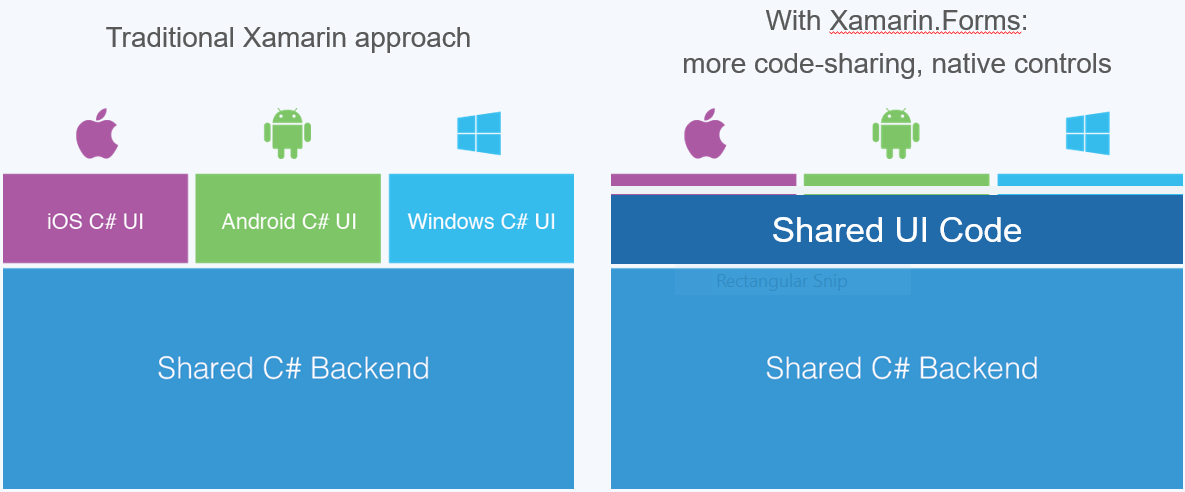
\includegraphics[width=1\hsize]{fig/xamarin}
\caption{architektura platformy Xamarin, \emph{Źródło: https://dab1nmslvvntp.cloudfront.net/wp-content/uploads/2016/02/1456296251XamVsXF.png}}
\end{figure}
\newpage

\section{Zbiór testowy}

W uczeniu maszynowym istnieje wiele metod testowania skuteczności klasyfikatorów. W pracy zawarto metodę losowego podziału na zbiory treningowe i testowe. Oznacza to, iż zbiór danych jest dzielony na dwie części. Uczenie klasyfikatora przebiega z wykorzystaniem zbioru treningowego, natomiast w celu sprawdzenia generalizacji klasyfikatora wykorzystywana jest testowa część danych\cite{19}. Metoda ta wydaje się być najbardziej zbliżona do rzeczywistości. Wadą w tym wypadku jest ograniczenie ilości danych treningowych, co w przypadku, gdy do dyspozycji jest niewielka liczba próbek lub występują ograniczenia sprzętowe, prowadzi do pogorszenia skuteczności klasyfikatora.

\section{Skuteczność klasyfikacji}

Używając zbioru treningowego stworzonego za pomocą narzędzia przedstawionego w sekcji 1.2 oraz klasyfikatorów problemu rozpoznania znaków pisma odręcznego wybranych w rodziale pierwszym przeprowadzone zostaną badania wykorzystujące algorytmy wymienione w sekcjach 1.3, 1.4 oraz sieci neuronowe z sekcji 1.5 oraz 1.6. Badanie zostało oparte o zbiór testowy zawierający 3600 elementów, uzyskane zostały  nastepujące rezultaty: 

\begin{table}[!htb]
\begin{tabular}{|l|l|} \hline
Nazwa & Dokładność \\ \hline
\texttt{kNN} & 60\% \\ \hline
\texttt{Random Forest} & 50\% \\ \hline
\texttt{Sieć neuronowa} & 91\% \\ \hline
\texttt{CNN}     & 95\% \\ \hline
\end{tabular}
\caption{Wyniki badań skuteczności klasyfikatorów}
\end{table}

Następnie używając zbioru testowego z poprzednich badań wykonane zostało porównanie rozpoznań aplikacji korzystających z gotowych bibliotek

\begin{table}[!htb]
\begin{tabular}{|l|l|} \hline
Nazwa & Dokładność \\ \hline
\texttt Computer Vision API & 29\% \\ \hline
\texttt Tesseract API & 32\% \\ \hline
\end{tabular}
\caption{Wyniki badań skuteczności klasyfikatorów}
\end{table}

Według wyników badań, najlepszą metodą klasyfikacji znaków pisma odręcznego jest wykorzystanie konwolucyjnych sieci neuronowych proponowanych przez autora.

\section{Czas treningu}

Używając zbioru treningowego stworzonego za pomocą narzędzia przedstawionego w sekcji 1.2 oraz klasyfikatorów problemu rozpoznania znaków pisma odręcznego wybranych w rodziale 1 przeprowadzone zostaną badania wykorzystujące algorytmy wymienione w sekcjach 1.3, 1.4 oraz sieci neuronowe z sekcji 1.5 oraz 1.6. Badanie zostało oparte o zbiór testowy zawierający 3600 elementów. Uzyskane zostały nastepujące rezultaty: 

\begin{table}[!htb]
\begin{tabular}{|l|l|l|} \hline
Nazwa & Czas(sekundy) \\ \hline
\texttt{kNN} & 12.3 \\ \hline
\texttt{Random Forest} & 9 \\ \hline
\texttt{Sieć neuronowa} & 159 \\ \hline
\texttt{CNN}     & 3969 \\ \hline
\end{tabular}
\caption{Wyniki badań czasu treningu klasyfikatorów}
\end{table}

Testy zostały przeprowadzone na komputerze MacBook Pro
(Retina, 13-inch Early 2015), procesor 2,7 GHz Intel Core i5, pamięć 8GB 1867MHz DDR.

Badanie bibliotek uczenia maszynowego zostało pominięte ze względu na to, iż w procesie nie występuje etap treningu.

\section{Porównanie modeli danych}

W celu przeprowadzenia porównania modeli danych treningowych problemu rozpoznawania polskich znaków pisanych utworzono pięć różnych zbiorów danych. Każdy z nich posiada określoną ilość elementów każdego znaku oraz rozdzielczość w jakiej zapisano poszczególne obrazy. Badanie ma na celu sprawdzenie czy w warunkach mocno ograniczających przeprowadzanie treningu modelu, np. na urządzeniach mobilnych, istnieje znacząca różnica w wynikach. Trening przeprowadzono wykorzystując proponowaną przez autora splotową sieć neuronowa. Rezultaty uzyskane w poprzednich badaniach pokazały, iż posiada ona najlepsze parametry wymagane do przeprowadzenia takiego testu.

\begin{table}[!htb]
\begin{tabular}{|l|l|l|} \hline
Model & Ilość elementów & Rozdzielczość  \\ \hline
\texttt 1 & 72000 & 28 x 28 pikseli \\ \hline
\texttt 2 & 250000 & 28 x 28 pikseli \\ \hline
\texttt 3 & 500000 & 28 x 28 pikseli \\ \hline
\texttt 4 & 750000 & 28 x 28 pikseli \\ \hline
\texttt 5 & 125000 & 32 x 32 pikseli \\ \hline
\end{tabular}
\caption{Dane wejściowe - porównanie modeli danych}
\end{table}

Wyniki treningu poszczególnych modeli, dla liczby iteracji równej 5000, do testu skuteczności został użyty zbiór testowy używany w poprzednich badaniach. Skuteczność przedstawiona w wynikach testu to procent prawidłowej klasyfikacji przy użyciu zbioru testowego.

\begin{table}[!htb]
\begin{tabular}{|l|l|l|} \hline
Model & Skuteczność & Czas treningu  \\ \hline
\texttt 1 & 90\% & 1h 32m \\ \hline
\texttt 2 & 88\% & 4h 51m \\ \hline
\texttt 3 & 94\% & 6h 02m \\ \hline
\texttt 4 & --- & --- \\ \hline 
\texttt 5 & 92\% & 2h 42m \\ \hline
\end{tabular}
\caption{Wyniki - porównanie modeli danych}
\end{table}

Badanie bibliotek uczenia maszynowego zostało pominięte ze względu na to, iż w procesie nie występuje etap treningu.
\newpage

\section{Rozmiar modelu a skuteczność terningu}

Z przeprowadzonych badań wynika, iż skuteczność treningu w pewnym stopniu zależna jest od ilości danych zawartych w zbiorze treningowym. Wszystkie porównania przeprowadzane były w warunkach domowych, co oznacza wysokie ograniczenia zasobów pamięci RAM, CPU oraz GPU. Trening na największym zbiorze danych nie był w stanie uruchomić się na środowisku testowym ponieważ zasoby potrzebne na operacje na macierzach wykonywane są w pamięci RAM, która jest znacznie ograniczona. 

Jednak z obserwacji wynika, iż im bardziej precyzyjne są dane zawarte w modelu, tym lepszy wynik końcowy treningu sieci neuronowych.

Małe modele danych, czyli takie, których trening oparty był na zbiorze treningowym o małej ilości elementów idealne są do celów sprawdzenia czy istnieje poprawa jakości wyodrębnionych cech poszczególnych obrazów i czy klasyfikacja zbioru testowego przyniesie lepsze wyniki.

\chapter{Podsumowanie i wnioski}

Wyniki otrzymane przez autora pokazują przewagę sieci neuronowych nad algorytmami z klasy regresji nieparametrytcznej lub teorii decyzji. Jeśli rozpatrywany jest model danych zawierający duży zbiór informacji, należy go odpowiednio przygotować, aby zawarte w nim właściwości jak najbardziej nadawały się do przetworzenia przez klasyfikator. 

Równie ważnym aspektem uczenia maszynowego jest posiadany sprzęt na którym klasyfikatory będą przeprowadzały trening modelu. Proces przebiegu treningu na domowym laptopie jest znacznie gorszy, niż na profesjonalym serwerze zaopatrzonym w technologię CUDA, czyli karty graficzne oferujące możliwość wykonywania obliczeń równoległych, które utylizują moc oferowaną przez procesory graficzne. W przeciwnym razie modele podczas treningu zapisywane są w pamięci podręcznej systemu, która przy dużym rozmiarze modelu, często przepełnia się. Efektem tego jest zmarnowany czas oraz zasoby.

\section{Uczenie maszynowe w aplikacjach mobilnych}

Wykorzystywanie technik uczenia maszynowego, czy są to algorytmy typu Random Forest, czy też sieci neuronowe, wymagają olbrzymich zasobów sprzętowych. W związku z tym urządzenia mobilne, których moc obliczeniowa nie może równać się z komputerami klasy PC czy klastrów procesorów graficznych nie nadają się do treningów. Istniejące gotowe rozwiązania jak na przykład przedstawione w pracu usługi Cognitive Services firmy Microsoft idealnie pasują do rynku aplikacji mobilnych, ponieważ wszystkie obliczenia związane z klasyfikacją znajdują się po stronie serwera. Wadą tego rozwiązania jest natomiast brak ingerencji w modele danych oraz brak jakiejkolwiek personalizacji, który mógłby pomóc w rozwiązaniu problemu.

Idealnym rozwiązaniem, również wykorzystanym w tej pracy przez autora jest połączenie mocy obliczeniowej komputerów PC lub laptopów by wytrenować odpowiedni model danych realizujący problem, a następnie stworzenie aplikacji webowej, która implementowałaby określony interfejs, tak aby była możliwość konsumowania go po stronie aplikacji mobilnej. W ten sposób zyskujemy niezawodność po stronie mobilnej oraz personalizacje i wgląd w model danych po stronie serwera.

\section{Najlepsza metoda rozpoznawania pisma odręcznego}

W pracy przedstawionej przez autora zostało zaprezentowanych kilka metod klasyfikacji
danych problemu rozpoznawania znaków pisma odręcznego oraz dwie
biblioteki umożliwiające błyskawiczne rozpoznanie obrazka bez konieczności posiadania
specjalistycznej wiedzy z zakresu uczenia maszynowego.
Według badań zawartych w rozdziale 3, najlepszym istniejącym sposobem rozwiązania
zadanego przez autora problemu jest wykorzystanie konwolucyjnych sieci
neuronowych. Model danych odgrywa najważniejszą role przy podejmowaniu
próby klasyfikacji znaków pisma odręcznego, gdyż elementy w nim zawarte powinny
jak najbardziej odzwierciedlać rzeczywiste cechy liter oraz cyfr.

\section{Zalety aplikacji wieloplatformowych}

\begin{itemize}
\item
Xamarin bazowo unifikuje przede wszystkim serwerową część aplikacji. Jeśli tworzymy aplikacje z rozbudowaną logiką biznesową, to warto ją pisać tylko raz. Xamarin na pewno w tym pomoże
\item
Jeśli layout aplikacji opiera się o standardowe elementy i wzorce, to warto użyć Xamarin.Forms, który obsługuje kilkadziesiąt kontrolek, które później mapowane są na natywne rozwiązania
\item
Jeśli konieczne jest posiadanie osobnego zestawu programistów na każdą platformę, to również warto dać szansę Xamarinowi. Nawet podejście natywne można w całości napisać w języku C\#. Xamarin mapuje 100\% API z platform Android oraz iOS
\item
Jeśli programista posiada doświadczenie w jakiejkolwiek technologii opierającej na XAMLu (WPF, Silverlight, Universal Apps, UWP), to również w tej sytuacji nie powinien mieć problemów z programowaniem w Xamarin.Formsie
\item
Pod Xamarina można programować w Visual Studio [Community] dla Windows lub Xamarin Studio dla OS X
\item
Kod źródłowy całego rozwiązania dostępny jest na GitHubie
\end{itemize}

\section{Wady aplikacji wieloplatformowych}

\begin{itemize}
\item
Podejście Forms zazwyczaj nie pozwala na napisanie całej aplikacji. Część kodu i tak musi być pisania z użyciem dedykowanych konstrukcji warunkowych, a w przypadku złożonych interfejsów, może to być większa część kodu
\item
Do pracy z Xamarinem wymagana jest również przynajmniej bazowa znajomość C\#. W podejściu Xamarin.Forms, trzeba się również nauczyć XAMLa.
\item
Ponadto przy wydaniu każdej nowej wersji wspieranych systemów, należy czekać na wrappery. Oczywiście w chwili obecnej pojawiają się one praktycznie natychmiast.
\item
Xamarin bywa również niestabilny. Zdarzają się wersje lepsze i gorsze. Czasami pojawiają się problemy w sytuacji gdy odpalamy solucję przygotowaną w Visual Studio na Macu i odwrotnie. Zdarzają się również inne błędy.

\end{itemize}

% zakończenie
\summary

Problem OCR (ang. Optical Character Recognition) należy do jednej z najbardziej popularnych grup w branży zgłebiania danych i uczenia maszynowego. Dzięki gotowym bibliotekom, które oferowane są przez firmy takie jak Microsoft lub Amazon pozwalają programistom na budowę funkcjonalności w swoich programach, które wykonują rozpoznanie znaków w czasie rzeczywistym bez potrzeby pozyskiwania specjalistycznej wiedzy na temat algorytmów oraz sieci neuronowych. Natomiast, jeśli rozpatrywany jest konkretny przypadek np. problem rozpoznawania znaków pisma odręcznego, istniejące rozwiązania moga nie być wystarczające, ponieważ osiągane przez nie wyniki są zbyt niskie by stosować je na środowiskach produkcyjnych.

Celem pracy autora było zaprezentowanie istniejących rozwiązań pozwalających na szybkie przeprowadzenie rozpoznania znaków pisma odręcznego oraz przedstawienie własnej implementacji sieci neuronowej, która rozwiązuje problem ten problem. 

Wynikiem pracy jest webservice dostępny do użytku ogólnego oraz aplikacja wieloplatformowa, która pozwala sklasyfikować dowolną literę bądź cyfrę. Skuteczność wytworzonego modelu na podstawie propozycji sieci neuronowej autora znacząco poprawia istniejące implementacje dostępne do użytku. Cel pracy został zrealizowany.

Cel pracy, czyli przedstawienie własnego rozwiązania mogącego w przyszłości posłużyć do rozpoznawania znaków pisma odręcznego w formularzach został zrealizowany. Autor pracy zamierza rozszerzyć funkcjonalność zawartą w publikacji, aby mogła ona posłużyć rozpoznawaniu pisma na różnego rodzaju formularzach.

% literatura (obowiązkowo):
\bibliographystyle{unsrt}
\bibliography{xml}

\begin{thebibliography}{9}

\bibitem{1}
  Brandewinder,
  Mathias,
  2015,
  \emph{Machine Learning Projects for .NET Developers},
  Apress,
  ISBN: 978-1-4302-6766-9.

\bibitem{2}
  M. Narasimha,
  Murty,
  2015,
  \emph{Introduction to pattern recognition and machine learning},
  World Scientific Publishing Co. Pte. Ltd,
  ISBN: 978-9-814-33545-4 .  

\bibitem{3}
  Kirk,
  Matthew,
  2015,
  \emph{Thoughtful Machine Learning},
  O'Reilly,
  ISBN: 978-1-449-37406-8.
  
\bibitem{4}
  Troelsen,
  Andrew,
  2011,
  \emph{Język C\# 2010 i platforma .NET 4},
  PWN,
  ISBN: 978-83-01-16666-3.
  
\bibitem{5}
  Norton,
  Peter,
  Samuel,
  Alex,
  Aitel,
  David,
  2005,
  \emph{Od podstaw Python},
  Wydawnictwo HELION,
  ISBN: 83-246-0528-2.  
  
\bibitem{6}
  Petzold,
  Charles,
  2016,
  \emph{Creating Mobile Apps with Xamarin.Forms},
  Microsoft Press,
  ISBN: 978-1-5093-0297-0.  

\bibitem{7}
  https://www.nist.gov/srd/nist-special-database-19
  (Dostęp 22 maja 2017r.)

\bibitem{8}
  https://github.com/mathias-brandewinder/machine-learning-projects-for-dot-net-developers
  (Dostęp 22 maja 2017r.)
  
\bibitem{9}
  https://azure.microsoft.com/en-us/services/cognitive-services/
  (Dostęp 22 maja 2017r.)

\bibitem{10}
  https://github.com/tesseract-ocr/tesseract
  (Dostęp 22 maja 2017r.)
  
\bibitem{11}
  http://shyamalapriya.github.io/digit-recognition-using-k-nearest-neighbors/,
  (Dostęp 22 maja 2017r.)

\bibitem{12}
  http://neuralnetworksanddeeplearning.com/chap1.html,
  (Dostęp 22 maja 2017r.)

\bibitem{13}
  http://deblivingdata.net/machine-learning-the-digit-recognition-problem/,
  (Dostęp 22 maja 2017r.)

\bibitem{14}
  http://cs231n.github.io/convolutional-networks/, 
  (Dostęp 22 maja 2017r.)

\bibitem{15}
  https://www.xamarin.com/platform, 
  (Dostęp 22 maja 2017r.)

\bibitem{16}
  https://www.tensorflow.org/api\_docs/, 
  (Dostęp 22 maja 2017r.)

\bibitem{17}
  http://scikit-learn.org/, 
  (Dostęp 22 maja 2017r.)  

\bibitem{18}
  http://www.emgu.com/wiki/index.php/Main\_Page, 
  (Dostęp 22 maja 2017r.)
  
\bibitem{19}
  https://stats.stackexchange.com/questions/19048/what-is-the-difference-between-test-set-and-validation-set, 
  (Dostęp 22 maja 2017r.)

\bibitem{20}
  https://en.wikipedia.org/wiki/Optical\_character\_recognition, 
  (Dostęp 22 maja 2017r.)

\bibitem{21}
  http://opencv.org,
  (Dostęp 27 maja 2017r.)

\end{thebibliography}

\oswiadczenie

\end{document}